\documentclass{article}

\usepackage{geometry}
\usepackage{makecell}
\usepackage{array}
\usepackage{multicol}
\usepackage{setspace}
\usepackage{changepage}
\usepackage{booktabs}
\usepackage{multicol}
\usepackage{wrapfig}
\usepackage{cancel}
\usepackage[explicit]{titlesec}
\usepackage{hyperref}
\usepackage{graphicx}
\usepackage{xcolor}
\usepackage{cprotect}
\usepackage{float}
\newcolumntype{?}{!{\vrule width 1pt}}
\newcommand{\paragraphlb}[1]{\paragraph{#1}\mbox{}\\}
\renewcommand{\contentsname}{Inhaltsverzeichnis:}
\renewcommand\theadalign{tl}
\setstretch{1.10}
\setlength{\parindent}{0pt}

\titleformat{\section}
  {\normalfont\Large\bfseries}{\thesection}{1em}{\hyperlink{sec-\thesection}{#1}
\addtocontents{toc}{\protect\hypertarget{sec-\thesection}{}}}
\titleformat{name=\section,numberless}
  {\normalfont\Large\bfseries}{}{0pt}{#1}

\titleformat{\subsection}
  {\normalfont\large\bfseries}{\thesubsection}{1em}{\hyperlink{subsec-\thesubsection}{#1}
\addtocontents{toc}{\protect\hypertarget{subsec-\thesubsection}{}}}
\titleformat{name=\subsection,numberless}
  {\normalfont\large\bfseries}{\thesubsection}{0pt}{#1}

\hypersetup{
    colorlinks,
    citecolor=black,
    filecolor=black,
    linkcolor=black,
    urlcolor=black
}

\geometry{top=12mm, left=1cm, right=2cm}
\title{\vspace{-1cm}Datenstrukturen und Algorithmen}
\author{Andreas Hofer}

\begin{document}
	\maketitle
	\tableofcontents
	\section{Einführung}
	Datenstrukturen und Algorithmen sind ein essenzieller Bestandteil moderner Systeme, da diese die Geschwindigkeit der meisten Operationen um ein Vielfaches erhöhen. Ob bei Netzwerkrouting, Rendering oder der Kryptographie, Algorithmen finden in allen Facetten des digitalen Bereichs Anwendung. \\
	In der grundlegendsten Form ist ein Algorithmus ein fest beschriebener Weg zur Lösung eines Problems in ihrer allgemeinen Form. Zwei Binärzahlen werden beispielsweise addiert, indem beide Zahlen von rechts nach links verglichen werden und dann anhand der Zahlen diese eine neue Zahl bilden und eventuell eine Zahl in das nächste Register überführt wird. Ein Algorithmus beschreibt also zwar den Lösungsweg für ein Problem aber nicht dessen Implementation. Zusätzlich hat ein Algorithmus stets für eine Eingabe eine eindeutige Ausgabe. \\
	Jedoch muss beachtet werden, dass nicht jedes Problem algorithmisch lösbar (Wie das Halteproblem \hyperref{/../Semester 1/GDI1/GDI.pdf}{halteproblem1}{halteproblem2}{Siehe GDI1}) ist und auch nicht jedes Problem ist praktisch berechenbar (Wie NP-Komplette Probleme [TODO LINK GDI]). \\
	Ein Algorithmus hat einige Eigenschaften:
	\begin{itemize}
		\item{Terminiertheit}
		\begin{itemize}
			\item{Eine Eingabe führt nach einer endlichen Anzahl an Schritten zu einer Ausgabe oder einem Abbruch}
		\end{itemize}
		\item{Finitheit}
		\begin{itemize}
			\item{Es gibt eine endliche Menge an Befehlen}
		\end{itemize}
		\item{Effektivität}
		\begin{itemize}
			\item{Die Auswirkung jedes Befehls innerhalb des Algorithmus ist eindeutig}
		\end{itemize}
		\item{Determiniertheit}
		\begin{itemize}
			\item{Die gleichen Eingaben führen zur gleichen Ausgabe}
		\end{itemize}
		\item{Determinismus}
		\begin{itemize}
			\item{Bei gleichen Eingaben wird auch der selbe Lösungsweg genommen.}
			\item{Ein Algorithmus kann determiniert aber nicht determistisch sein, wenn darin Zufallselemente vorkommen}
		\end{itemize}
	\end{itemize}
	Zusätzlich zur bereits bekannten Zeitkomplexität in der O-Notation (Siehe GDI [TODO GDI Link]) gibt es auch Speicherkomplexität, was beschreibt wie viel zusätzlichen Speicherplatz ein Algorithmus benötigt um das Problem zu lösen. Einen Algorithmus welcher keinen zusätzlichen Speicherplatz benötigt nennt man "In-Place". \\
	\section{Insertion Sort}
	Insertion Sort ist einer der simpelsten Sortieralgorithmen mit jedoch einer relativ hohen Laufzeit. Er funktioniert, indem er stets von links nach rechts ein Array durchläuft und jeweils eine niedrigere mit einer höheren Zahl vertauscht. Diese Zahl wird so lange vertauscht, bis die linke Zahl kleiner ist als die rechte. Danach wird der Zähler nach rechts verschoben und die nächste Zahl verglichen bis man an das Ende des Arrays kommt. \\
	\subsection{Pseudocode}
	Angenommen man hat ein Array [8, 6, 9, 5], dann würde der Prozess in ewta so aussehen: \\
	\begin{tabular}{| l | l | l | l | c | c |}
		\toprule
		i & key & j & A[j] & $A[j]>$key \& $j>0$ & A \\ \midrule
		2 & 6 & 1 & 8 & $8>6\&1>0$ -> True & $[-_1, \textcolor{red}{8}_2, 9_3, 5_4]$ \\
		- & - & 0 & - & - -> False & $[\textcolor{red}{6}_1, 8_2, 9_3, 5_4]$ \\ \hline
		3 & 9 & 2 & 8 & $8>9\&2>0$ -> False & $[6_1, 8_2, 9_3, 5_4]$ \\ \hline
		4 & 5 & 3 & 9 & $9>5\&3>0$ -> True & $[6_1, 8_2, -_3, \textcolor{red}{9}_4]$ \\
		- & - & 2 & 8 & $8>5\&2>0$ -> True & $[6_1, -_2, \textcolor{red}{8}_3, 9_4]$ \\
		- & - & 1 & 6 & $6>5\&1>0$ -> True & $[-_1, \textcolor{red}{6}_2, 8_3, 9_4]$ \\
		- & - & 0 & - & - -> False & $[\textcolor{red}{5}_1, 6_2, 8_3, 8_4]$ \\
		\bottomrule
	\end{tabular}
	\section{Analyse von Algorithmen}
	Die Analyse von Algorithmen ist wichtig um deren Effizienz finden und sie vergleichen zu können. Um diese zu vergleichen wird eine Abstraktion eines Rechners verwendeten, welcher eine spezifische Konfiguration hat. Dieser theoretische Rechner hat folgende Eigenschaften:
	\begin{itemize}
		\item{Es existiert 1 Prozessor, welcher jeweils einen Befehl sequenziell abarbeitet}
		\item{Jede Zahl im Programm passt in eine Speichereinheit}
		\item{Speicherzugriff ist immer gleich schnell}
		\item{Primitive Operationen dauern immer gleich lang. Primitive Operationen sind:}
		\begin{itemize}
			\item{Eine Zuweisung \texttt{a = b}}
			\item{Eine arithmetische Operation wie Addition, Subtraktion, etc \texttt{a + b}}
			\item{Vergleichsoperatoren wie größer, kleiner oder gleich \texttt{a > b}}
			\item{Befehle zur Ablaufsteuerung wie \texttt{if}, \texttt{else} oder \texttt{while} \texttt{if (a == b)}}
		\end{itemize}
	\end{itemize}
	\subsection{Laufzeitberechnung}
	\subsubsection{Sequenz}
	Die Laufzeit einer Sequenz ohne Schleifen wird anhand ihrer Aktionen summiert. Man kann eine arithmetische Operation mit Zuweisung als eine oder zwei Aktionen sehen.
	\begin{figure}[H]
	\centering
	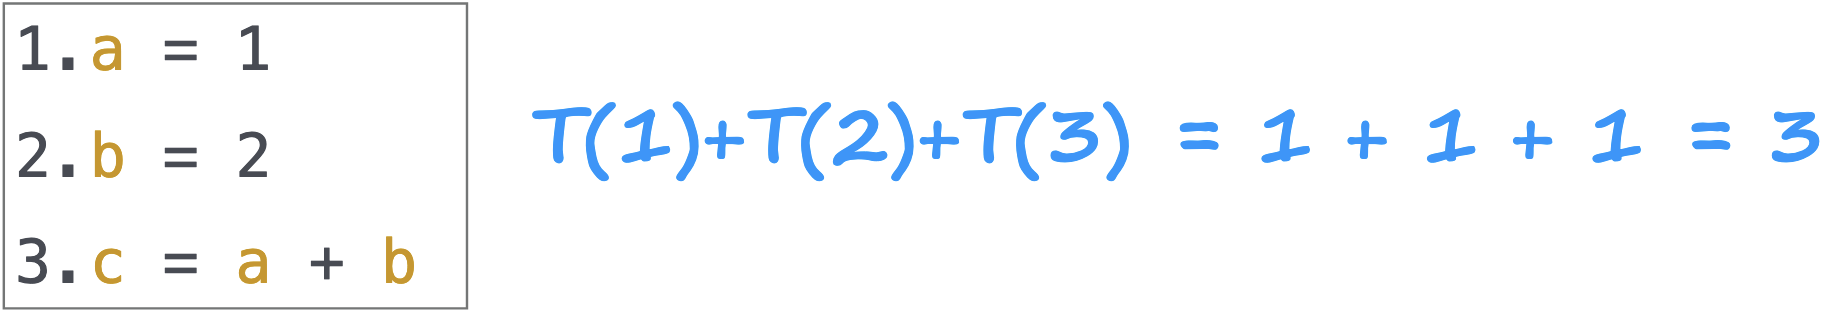
\includegraphics[width=0.48\textwidth]{Bilder/sequence.png}
	\caption{Summierung einer Sequenz an Befehlen}
	\end{figure}
	\subsubsection{Schleifen}
	Bei einer Schleife wird die Menge an Sequenzen mit der Anzahl an Schleifendurchläufen multipliziert. Man muss beachten, dass ein Programm eine Schleife immer noch ein Mal evaluiert, before sie beendet wird, weshalb bei einer Schleife mit 2 Durchläufen die Schleife 3 Mal evaluiert wird (Ein Mal am Anfang, ein Mal nach der Erhöhung und ein Mal am Ende).
	\begin{figure}[H]
	\centering
	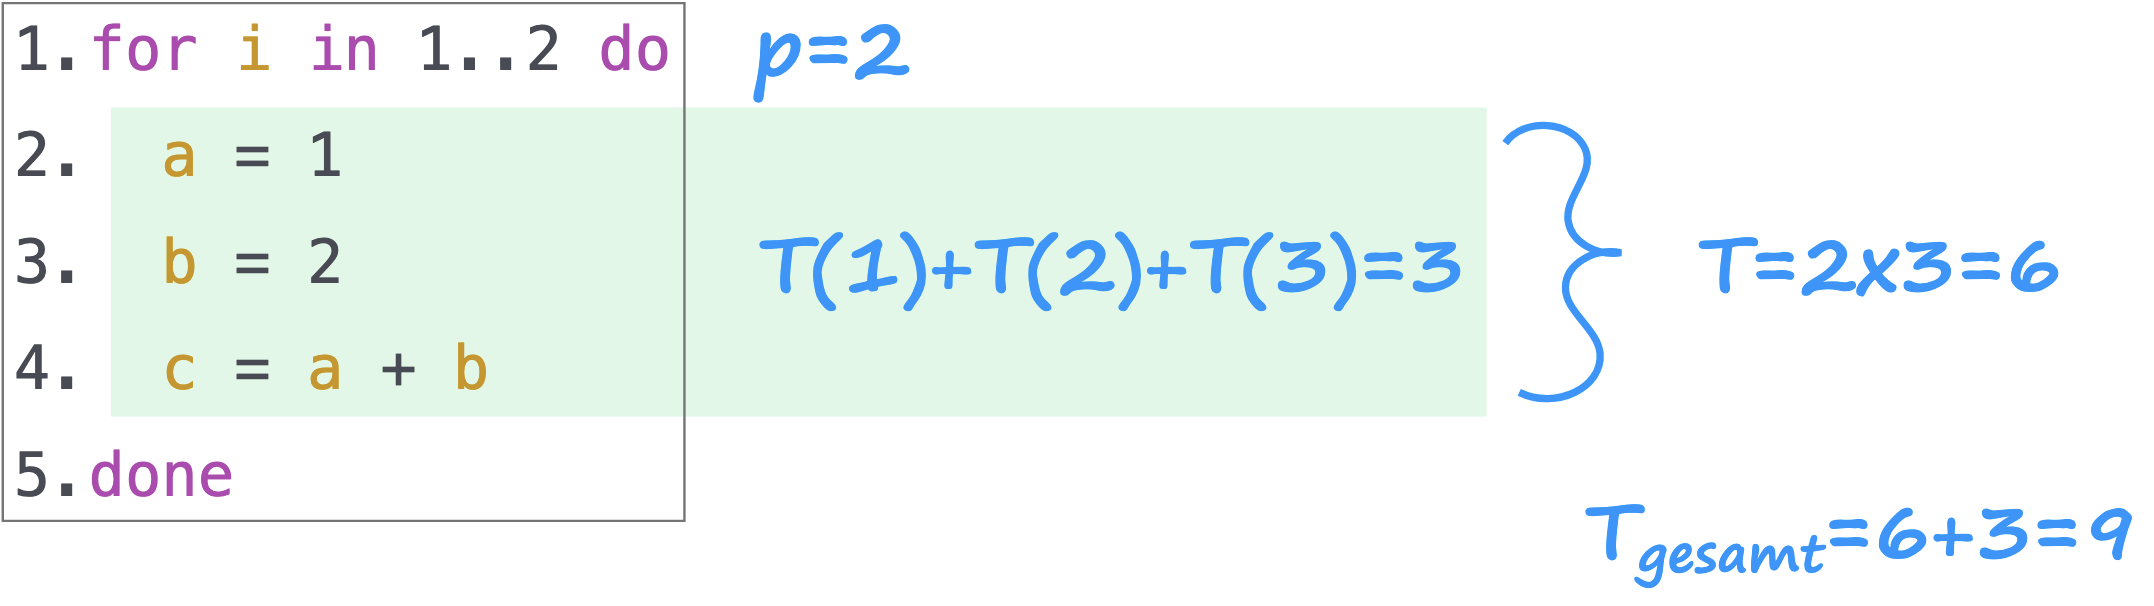
\includegraphics[width=0.48\textwidth]{Bilder/loop.png}
	\caption{Summierung einer Sequenz an Befehlen}
	\end{figure}
	\subsubsection{Verschachtelte Schleifen}
	Wenn Schleifen verschachtelt werden, erhöht sich die Anzahl an Schritten um ein vielfaches. Da eine Schleife mit 5 Ausführungen, welche in einer anderen Schleife mit 10 Ausführungen sitzt, bei jedem der 10 Durchläufe 5 Mal durchlaufen wird muss man die Schritte einer Schleife mit der äußeren Schleife multiplizieren um die Anzahl der Schritte zu erhalten. Also muss man die Schritte in einer Schleife mit der Anzahl an Wiederholungen multiplizieren und danach wiederum mit der Anzahl an Wiederholungen der äußeren Schleife.
	\begin{figure}[H]
	\centering
	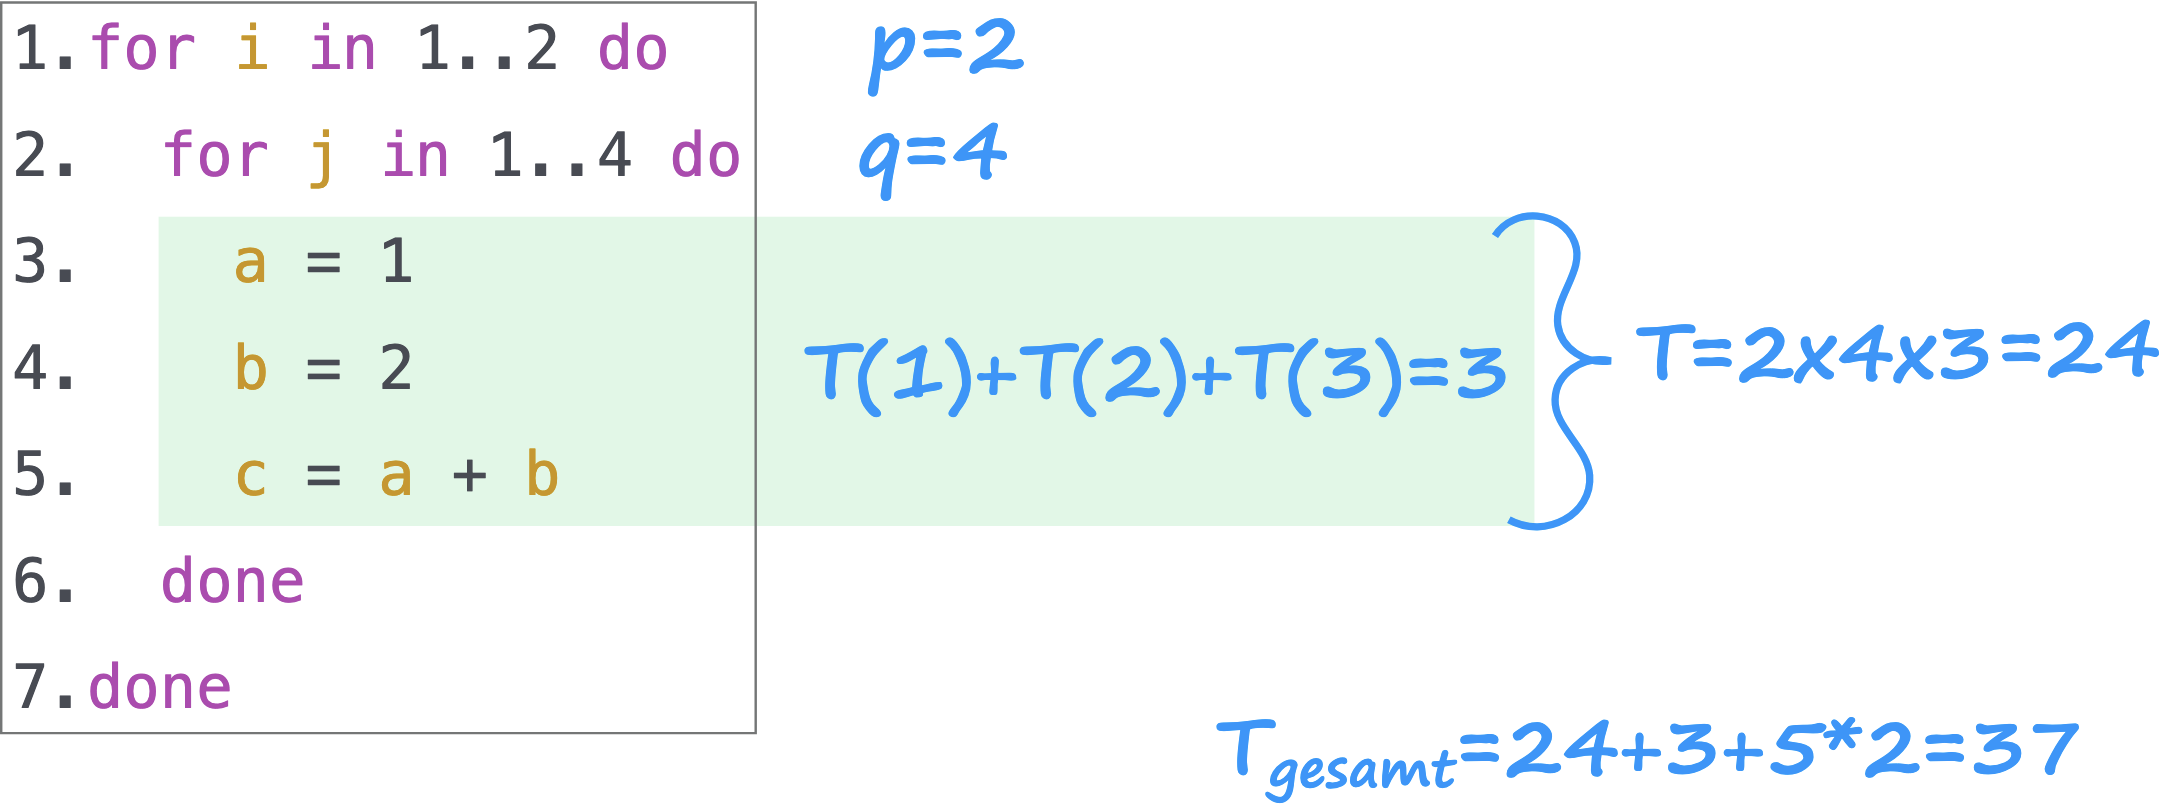
\includegraphics[scale=0.20]{Bilder/nested.png}
	\caption{Laufzeit einer verschachtelten Schleife}
	\end{figure}
	\subsection{Best Case}
	Der Best Case tritt auf, wenn der Algorithmus die geringstmögliche Anzahl an Schritte abhängig von der Eingabe durchläuft. Bei dem Insertion Sort tritt das auf, wenn das Array bereits sortiert ist. \\
	Da trotzdem das Array ein Mal durchlaufen werden muss um dessen Sortiertheit zu überprüfen, ist die Laufzeit n-1 ($\sum_{i=2}^{n}t_i$ => $\sum_{i=2}^{n}1$ => (n-1)) \\
	$T(n)=c_1n+c_2(n-1)+c_3(n-1)+c_4(\sum_{i=2}^{n}t_i)+\cancel{c_5*\sum_{i=2}^{n}(t_i-1)}\cancel{+c_6*\sum_{i=2}^{n}(t_i-1)}+c_7(n-1)$ \\
	$c_1n+c_2(n-1)+c_3(n-1)+c_4(n-1)+c_7(n-1)=(c_1+c_2+c_3+c_4+c_7)n-(c_2+c_3+c_4+c_7)=c_x*n-c_y$ \texttt{Da es sich um einen linearen (cx*n) und einen konstanten (cy) Faktor handelt, dominiert der lineare und es handelt sich deshalb um eine Komplexität von O(n)}
	\subsection{Worst Case}
	Der Worst Case ist das Gegenteil des Best Case und gibt die Laufzeit des Algorithmus an, wenn er die höchstmögliche Arbeit volrichten muss um zum Ergebnis zu bekommen. Das geschieht im Insertion wenn das Array verkehrt sortiert ist, da dadurch jedes Element an das andere Ende des Arrays verschoben werden muss. In diesem Fall hat Insertion Sort eine Laufzeit von $n^2$. \\
	\subsection{Average Case}
	Der Average Case versucht die mittlere Performance eines Algorithmus zu berechnen. In den meisten Fällen ist der Average Case nur unmerklich besser als der Worst Case. Da man die durchschnittliche Verteilung der Inputarrays kennen muss, ist die Berechnung des Average Case relativ aufwändig und normalerweise nur relevant wenn der Worst Case sehr selten eintrifft.
	\section{Landau Notation}
	Wie bereits in Grundlagen der Informatik besprochen, beschreibt die Landau-Notation (O-Notation) die geringste obere Schranke eines Algorithmus. Zur Bestimmung der Laufzeit muss man so stets immer den variablen Teil der Laufzeit mit der höchsten Notation nehmen und diesen als dessen O-Notation angeben. Beispiele sind: \\
	$f(n)=3n^2+n\in O(n^2)$ \\
	$f(n)=5^n+n^2-5\in O(5^n)$ \\
	$f(n)=2\log(5n)n^2+4(\log(n))\in O(log(n)n^2)$ \\
	$f(n)=-2n^2+50n-4\in O(n)$ \texttt{-> Nur ein theoretisches Beispiel. Ein Teil eines Algorithmus kann keine negative Laufzeit haben.} \\
	\subsection{Zugehörigkeit}
	Man kann diese Zugehörigkeit des Grenzwerts jedoch auch direkt berechnen indem man den Limes verwendet: $\lim_{n\to\infty}\frac{f(n)}{g(n)}=K, 0\leq K\leq \infty$ \\
	Wenn man also zwei Funktionen vergleicht kann man diese mittels des limes gegenüberstellen um den schneller ansteigenden zu bestimmen: \\
	$f(n)=42, g(h)=n*\pi, f(n)\in O(g(n))?$ \texttt{Ist f(n) Teil der oberen Schranke?} \\
	$\lim_{n\to\infty}\frac{42}{n*\pi}=0=K$ \texttt{->} $0\leq K < \infty$ \texttt{42 ist also Teil der Schranke} \\
	\subsection{Untere Schranke}
	Während man die obere Schranke die O-Notation nennt, ist die untere Schranke die $\Omega$-Notation. Die Definition ist die selbe, außer, dass die Funktion f(n) stets kleiner oder gleich sein muss als größer. Die Berechnung des Grenzwerts ist ebenfalls der selbe, nur die Einschränkung ist anders, sodass K größer als 0 und kleiner gleich unendlich sein muss: $0 < K \leq \infty$.
	\subsubsection{Berechnung:}
	$2n^2-3n+5\in \Omega(n)?, 0<K\leq\infty$ \\
	$\lim_{n\to\infty}\frac{2n^2-3n+5}{n}=\lim_{n\to\infty}\frac{2n^2}{n}-\lim_{n\to\infty}\frac{3\cancel{n}}{\cancel{n}}+\lim_{n\to\infty}\frac{5}{n}=\infty-3+0=\infty=K$ \texttt{-> 2$n^2$-3n+5 hat Omega(n) als untere Schranke}
	\subsection{Exakte Schranke}
	Zusätzlich existiert noch die Exakte Schranke, auch $\Theta$-Schranke genannt. Während die vorherigen Schranken die obere und untere Grenze suchen, bezeichnet die exakte Schranke die Fläche dazwischen. So muss f(n) stets zwischen der oberen und unteren Schranke existieren. Die Berechnung des Grenzwerts ist wiederum der selbe mit einem anderen Grenzwert, welcher strikt zwischen 0 und unendlich sein muss (Ohne die Erlaubnis gleich wie eine der beiden Seiten zu sein): $0 < K <\infty$
	\subsubsection{Berechnung:}
	$2^n+n^2\in\Theta{2^n}?, 0<K<\infty$ \\ 
	$\lim_{n\to\infty}\frac{2^n+n^2}{2^n}=\lim_{n\to\infty}\cancel{\frac{2^n}{2^n}}+\lim_{n\to\infty}\frac{n^2}{2^n}=1+0+1$
	\section{Datenstrukturen}
	Eine Datenstruktur ist eine Kollektion an Daten, welche geordnet abgespeichert werden. Da solche Datenstrukturen stets wiederum auf Algorithmen beruhen um Daten einzufügen, zu finden und wieder zu löschen, haben auch diese eine Laufzeit. Dabei bieten gewisse Strukturen bessere einfüge-, such- oder Löschzeiten. Eine Datenstruktur besteht deshalb stets aus den gespeicherten Daten sowie dessen Operationen. DS bieten auch oft weitere Operationen wie das i-te Element finden, die Anzahl der Elemente angeben oder den Nachfolger eines Elements zu finden. \\
	\subsection{Elementare Datenstrukturen}
	Es gibt vier elementare Datenstrukturen: Das Array (Lineares Feld), Linked List(Verkettete Liste), Stack (Keller- oder Stapelspeicher) und Queue (Warteschlange). Es gibt jedoch auch kombinierte Datenstrukturen wie zum Beispiel ein Array aus verketteten Listen. Also gibt es viele Arrays, welche jeweils auf das nächste Array zeigen. Diesen Vorgang nennt man auch nesting.
	\subsubsection{Array}
	Ein Array ist in der Lage mehrere Elemente des gleichen Basistyps abzuspeichern. Zugriff auf einzelne Elemente ist mittels des Index möglich. Das Array ist eine statische Datenstruktur, dessen Größe kann also nur ein Mal definiert werden und muss erneut generiert werden um dessen Größe zu erhöhen. Anders als andere Datenstrukture stehen die Daten eines Arrays stets nebeneinander. \\
	Die Zugriffszeiten für ein Array sind: \\
	\begin{tabular}{| l | l | l |}
		\toprule
		Operation & Laufzeit & Erklärung \\ \midrule
		Zugriff auf i-tes Element & O(1) & Da alle Elemente nebeneinander liegen können diese sofort angesprochen werden \\ \hline
		Suchen & O(n) & Da das Array linear iteriert werden muss um einen Wert zu finden. \\ \hline
		Einfügen/Löschen & O(n) & Da man das Array eventuell neu generieren muss. \\ \hline
		Speicherbedarf & O(n) & Jedes Element muss genau ein Mal abgespeichert werden.\\
		\bottomrule
	\end{tabular} \\
	Arrays finden Anwendung wenn eine Liste oder eine Matrize verwendet werden soll. Es ist besonders effizient, wenn man im Vorhinein weiß, wie groß das Array sein muss. Falls man einen Graphen oder ein zweidimensionales Array abbilden will, ist es auch praktisch ein Array zu verwenden. \\
	In Java kann man ein primitives Array mit eckigen Klammern generieren \texttt{int[] -> Generiert ein Array aus Integerwerten.}. Zusätzlich existieren zwei auf Arrays basierenden Collections: Die ArrayList und den Vector. Die ArrayList ist eine dynamische Version eines Arrays, welches neuen Speicher allokiert falls nötig, ohne das dies explizit angegeben werden muss. Vector ist eine ältere Version der ArrayList, welche thread-safe ist, also bei multithreading keine race-condition auslösen kann. \\
	\subsubsection{Linked List}
	Eine Linked List ist eine dynamische Datenstruktur in der jedes Element eine Referenz auf das nächste Element besitzt. Aus diesem Grund müssen die Daten nicht nebeneinander abgespeichert werden, sondern werden über die Pointer gefunden. Dadurch besteht auch keine Garantier, dass folgende Daten auch nebeneinander im Speicher liegen. \\
	Es gibt zwei Arten von Linked Lists: Single-Linked (Einfach verkettete) und Double-Linked (Dopplet-verkettete) Lists. Einfach verkettet Listen haben die Referenz nur in eine Richtung, wodurch man nicht zurückgehen kann. \\
	Die Zugriffszeiten für eine Linked List sind: \\
	\begin{tabular}{| l | l | l |}
		\toprule
		Operation & Laufzeit & Erklärung \\ \midrule
		Zugriff auf i-tes Element & O(n) & Da Pointer durchlaufen werden müssen um das Element zu finden. \\ \hline
		Suchen & O(n) & Da man wieder über die Pointer Elemente suchen muss. \\ \hline
		Einfügen/Löschen des Kopfes & O(n) & Da man das Element nur am Anfang einfügen muss \\ \hline
		Speicherbedarf & O(n) & Jedes Element benötigt zwar Pointer, ist jedoch trotzdem linear.\\
		\bottomrule
	\end{tabular} \\
	Double-Linked Lists besitzen ihre Referenz in beide Richtungen, wodurch man entweder nach vorne oder nach hinten gehen kann. Dadurch besitzt die Liste einen Head und einen Tail (Am Anfang und am Ende), wodurch an beide Enden ein Element angefügt werden kann. Dabei muss man jedoch beachten, dass die Pointer stets die richtigen Elemente als Ziel besitzen. \\
	Eine spezielle Art der Linked-List ist die Circular-List, in welche das letzte Element wiederum auf das erste zeigt, wodurch sie kein Ende besitzt. \\
	Eine Linked List ist sehr effektiv, wenn man nicht weiß, wie viele Elemente man haben wird, da dynamisch weitere hinzugefügt werden können. Bei der dynamischen Speicherverwaltung ist es auch nützlich, da man so die Menge an leeren und besetzten Elementen stets anpassen kann. \\
	In Java existiert eine LinkedList collection, welche eine Double-Linked List implementiert.
	\subsubsection{Stacks}
	Ein Stack (Auf Deutsch Stapel) ist eine dynamische Datenstruktur, bei welcher nur das oberste Element manipuliert werden kann. So kann man nur ganz oben ein Element hinzufügen (Push) und nur das oberste Element jeweils entfernen (Pop). Zusätzlich kann man mittels \texttt{peek} auch den Wert des obersten Elements auslesen ohne es zu entfernen. Dieses Prinzip nennt man auch LIFO, Last-In First-Out. \\
	Ein Weg einen solchen Stack zu implementieren ist mit einem Arrax, welches danach die Elemente sequentiell abspeichert. Dabei muss man jedoch beachten, dass ein Array stets eine statische Größe hat, ein Stack jedoch eigentlich eine dynamische Datenstruktur sein sollte. Nun könnte man jedes Mal, wenn die Maximalgröße erreicht wurde, die Größe des Arrays um 1 erhöhen, das ist jedoch eine sehr ineffiziente Operation da Arrays mit O(n) verschoben werden. Ein besserer Weg dies umzusetzen ist das sogenannte \texttt{Repeated Doubling}, wobei jedes Mal, wenn man die Maximalgröße erreicht hat, das Array in seiner Größe verdoppelt, wodurch das Array stets zwischen 50 und 75\% gefüllt ist. \\
	Ein besserer Weg zur Implementation ist die Linked List, da hierbei Elemente dynamisch aneinandergereiht werden. Und da man stets nur das erste Element braucht, ist auch die schlechtere Suchzeit der Linked List nicht relevant. \\
	Anwendungen des LIFO Prinzips wird für die Evaluierung von Semantik bei Programmiersprachen angewandt. Ebenfalls kann man Undo/Redo Operationen bei Programmen mittels Stack realisieren, da man so die letzten Operationen einfach auf den Stack legt. Um diese zurückgesetzten Operationen wieder zu revidieren kann man einen zweiten Stack machen, welcher Undo Operationen speichert. \\
	Bei einem Programmablauf gibt es auch den Call Stack, welcher die Reihenfolge von Methodenaufrufen abspeichert. \\
	Die Zugriffszeiten für einen Stack sind sind: \\
	\begin{tabular}{| l | l | l |}
		\toprule
		Operation & Laufzeit & Erklärung \\ \midrule
		Zugriff auf i-tes Element & O(n) [O($n^2$)] & \makecell[l]{Ein Element zu finden ist O(n) man muss jedoch eventuell Elemente \\ zurücklegen,  weshalb es O($n^2$) sein könnte} \\ \hline
		Suchen & O(n) [O($n^2$)] & Gleich wie bei dem Zugriff. Mit O(n) oder O($n^2$) \\ \hline
		Einfügen/Löschen des Kopfes & O(1) [O(n)] & Abhängig davon ob man das erste oder ein anderes Element anspricht \\ \hline
		Speicherbedarf & O(n) & Ein Element braucht genau eine Einheit an Speicher \\
		\bottomrule
	\end{tabular} \\
	\paragraphlb{Postfix}
	Ein weiterer wichtiger Anwendungszweck für Stacks ist die Evaluierung von Postfixoperationen. Normalerweise verwenden Menschen Infixoperationen, welche normale Mathematikausdrücke sind: \texttt{(3+7)*(5-1)+2}. Es heißt Infix, da die Operatoren zwischen den Zahlen stehen. Diese Rechnung kann man jedoch auch in Postfix anschreiben: \texttt{3 7 + 5 1 - * 2 +}. Was zuerst etwas unübersichtlich aussehen mag kann mit einem Stack sehr einfach von links nach rechts evaluiert werden. So wird stets zuerst der linkeste Wert eingelesen und auf den Stack gelegt. Wenn eine zahl eingelesen wird, wird sie auf den Stack gepusht. Wenn ein Operator eingelesen wird, wird dieser auf die obersten zwei Elemente des Stacks angewandt und zurück auf den Stack gelegt. \\
	Audruck: \texttt{2 4 1 + * 3 - = 2*(4+1)-3} \\
	\begin{tabular}{| l | l | l | l | l |}
		\toprule
		Input &Stackinhalt&&& \\ \midrule
		2 & 2 &&& \\ \hline
		4 & 2 & 4 && \\ \hline
		1 & 2 & 4 & 1 \\ \hline
		+ & 2 & 5 && \\ \hline
		* & 10 &&& \\ \hline
		3 & 10 & 3 && \\ \hline
		- & 7 &&& \\
		\bottomrule
	\end{tabular} \\
	\paragraphlb{Stacks in Java}
	Java implementiert auch Stacks, jedoch sollte man nicht die eingebaute Klasse \texttt{Stack} verwenden, da diese auf der Vector Klasse basiert. Stattdessen sollte man die Klasse \texttt{ArrayDeque} verwenden, da diese ein besseres Interface für eine Stackimplementation anbietet.
	\subsubsection{Queue}
	Eine weitere Datenstruktur ist die Queue, oder die Warteschlange. Hierbei wird zwar auch jedes Element ganz oben hinzugefügt, Elemente können jedoch nur von unten entfernt werden. Dies basiert auf dem FIFO (First-In First-Out) Prinzip. Eine Queue kann wiederum als Array oder als Linked List implementiert werden, wobei eine Linked List jedoch wiederum die effizientere Implementation darstellt. \\
	Queues werden vielfach angewandt, wenn man eine spezifische Reihenfolge für die Abarbeitung von Vorgängen benötigt. Wenn ein Server keine Kapazitäten verfügbar hat, kann er neue Anfragen in eine Ready Queue setzen und so neue Anfragen anhand ihrer Eingansgzeit verarbeiten. \\
	Eine alternative Implementation einer Queue ist die Priority Queue bei der man jedem Teilnehmer eine Priorität geben kann und so eventuell ein Element bevorzugten Zugang bekommt, obwohl dieser nicht an erster Stelle steht. \\
	Die Zugriffszeiten für einen Stack sind: \\
	\begin{tabular}{| l | l | l |}
		\toprule
		Operation & Laufzeit & Erklärung \\ \midrule
		Zugriff auf i-tes Element & O(n) & \makecell[l]{Jedes Element kann direkt wieder am Ende hinzugefügt werden, \\ also immer O(n)} \\ \hline
		Suchen & O(n) & Gleich wie bei Elementzugriff \\ \hline
		Einfügen/Löschen des Kopfes & O(1) [O(n)] & Entweder wieder erstes Element oder das n-te \\ \hline
		Speicherbedarf & O(n) & Ein Element braucht genau eine Einheit an Speicher \\
		\bottomrule
	\end{tabular} \\

	\subsection{Double Ended Queue (Deque)}
	Das bereits erwähnte \texttt{ArrayDeque} ist eine Implementation einer Double-Ended Queue, weshalb man von beiden Seiten ein Element hinzufügen oder entfernen kann, wobei die Pointer der Elemente auch in beide Richtung gehen. Somit ist das Hinzufügen und Entfernen, egal ob man eine Queue oder einen Stack implementiert, konstant.
	\newpage
	\section{Bäume}
	Bäume sehen in der Informatik etwas anders aus als man sich von echten Bäumen erwarten würde. Diese Art von Bäumen existieren jedoch auch außerhalb der IT wie zum Beispiel ein Stammbaum. Dabei entspringen von einer Quelle (Im Familienstammbaum der letzte Vorfahre) jeweils weitere Äste, von welchen wiederum weitere Äste entspringen. Auf diese Weise wird auch das Document Object Modle (DOM) in HTML (Siehe Web Technologies and Usability) generiert. Andere Anwendungen sind Web Crawler, welche das Internet anhand von Links auf Websiten durchforsten. Jeder aufgerufene Link auf einer Website ist eine Ebene unter dem Ursprung. Auch soziale Netzwerke können mit einem Baum dargestellt werden, da Benutzer stets untereinander verbunden sind. Auf die gleiche Weise funktioniert auch ein Network Broadcast wodurch jeder im gleichen Netzwerk (Der gleichen Hierarchie im Baum) die Nachricht erhält. \\
	Bisher waren alle beschriebenen Datenstrukturen lineare Datenstrukturen, wodurch diese eine intrinsische Reihenfolge hatten. So kann man an einem Ende beginnen und durchläuft am Ende jedes Element. Graphen und Bäume sind Nicht-Lineare Datenstrukturen wodurch bei einem Durchlauf nicht jedes Element erfasst werden muss. So kann ein Element mit mehr als einem Element verbunden sein. Bei einer Linked List, zum Beispiel, sind Elemente auch verbunden aber es gibt stets eine eindeutige Richtung.
	\subsection{Graphen}
	Graphen sind Bäume wo es keinen expliziten Anfang gibt, da dieser auch im Kreis gehen kann. Bei Graphen unterscheidet man zwischen gerichteten und ungerichteten Graphen. Ein ungerichteter Graph gibt keine Richtung der Verbindung an und kann so auf beiden Wegen verbunden sein. Gerichtete Graphen hingegen geben eine explizite Richtung an, wodurch diese auch nur in diese Richtung gehen kann.
	\begin{wrapfigure}{l}{0.5\textwidth}
	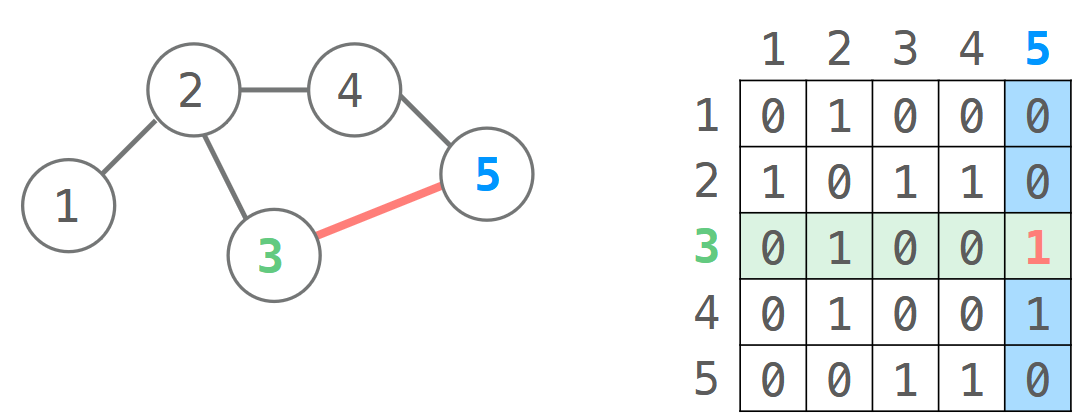
\includegraphics[width=0.5\textwidth]{Bilder/graph.png}
	\caption{Implementation eines Graphen in Java}
	\end{wrapfigure}
	\subsubsection{Java}
	Java bietet keine spezifische Datenstruktur an um einen Graphen darzustellen, jedoch kann man mit einem zweidimensionalen Array einfach eine definieren. Diese Datenstruktur nennt man Adjazenzmatrix oder Nachbarschaftsmatrix: \texttt{int Adjazenz [][]}. Dabei sind jeweils zwei Elemente miteinander anhand ihres Indexwertes verbunden. Elemente können entweder eine 1 oder eine 0 als Wert haben und diese sind dann in dieser Position mit dem anderen Element anhand ihres Indexes verbunden.
	\subsection{Baum}
	Ein Baum (oder Tree) ist eine speziellere Art von Graph wo keine Zylken enthalten sein können. Also darf ein Element nur nach unten aber nicht nach oben oder zur Seite verbunden sein. Das oberste Element eines Baumes nennt man dabei die Wurzel (root). Außer der Wurzel hat jedes Element einen Vorfahren, also ein Element das auf einer höheren Ebene liegt. Ein Vorfahre kann dabei beliebig viele Nachfolger haben. Elemente welche auf der selben Ebene liegen nennt man Geschiwster. Ein Element das nicht die Wurzel ist mit mindestens einem Nachfolger nennt man einen inneren Knoten und ein Element ohne Nachfolger nennt man Blätter. Für jeden Baum kann man auch einen Teilbaum definieren. Hierbei wird ein innerer Knoten als Wurzel eines neuen Baums definiert. Jeder innere Knoten in einem Baum kann als Teilbaum definiert werden. Ein Baum hat stets eine gewisse Menge an Ebenen, wobei die Wurzel auf der nullten Ebene (Ebene 0) ist. Jeder Nachfolger ist danach in einer weiteren Ebene.
	\subsubsection{Binärbaum}
	Ein Binärbaum ist eine spezielle Art von Baumstruktur. Hierbei darf jedes Element eines Baumes maximal zwei Kinder besitzen. Binärbäume sind in der Programmierung sehr nützlich da man viele Algorithmen effizient damit implementieren kann.
	\begin{wrapfigure}{l}{0.5\textwidth}
	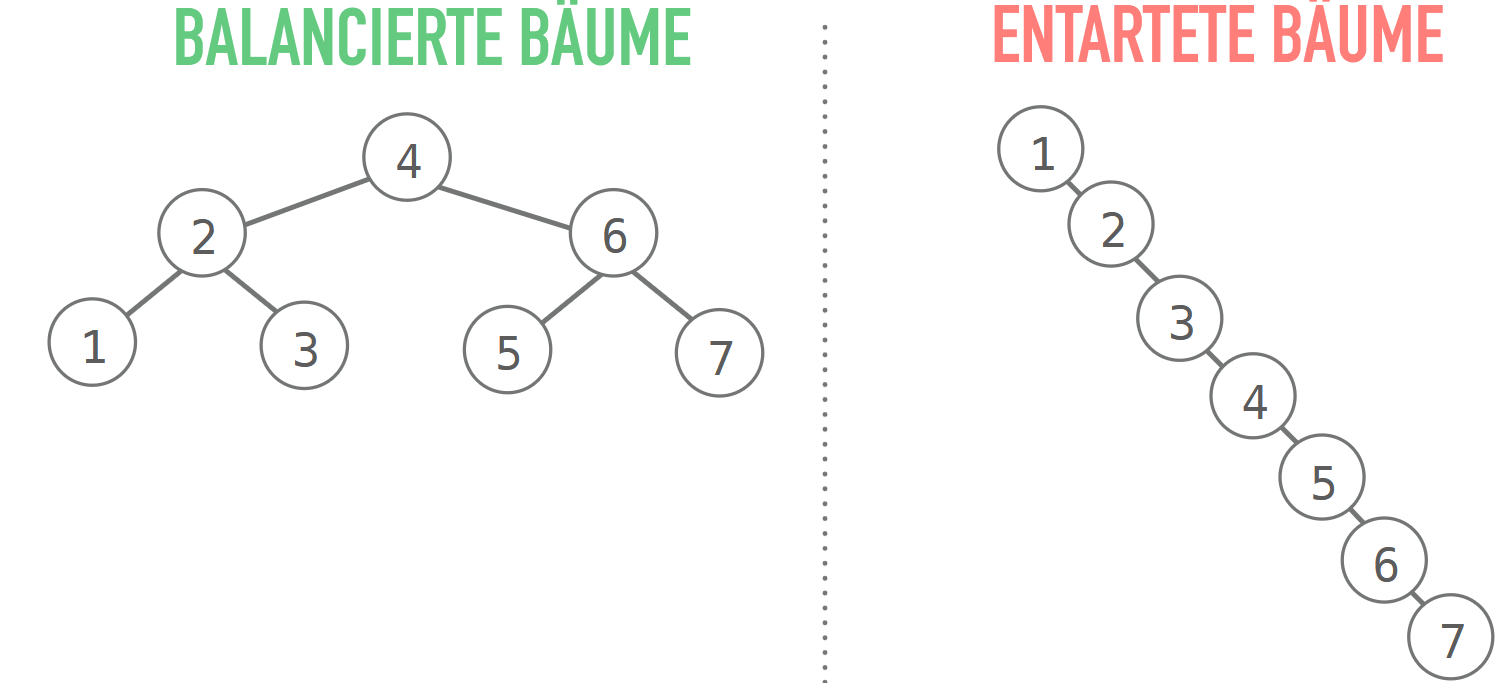
\includegraphics[width=0.5\textwidth]{Bilder/balanced.png}
	\caption{Jeweils ein balancierter und ein entarteter Baum}
	\end{wrapfigure}
	\subsubsection{Balancierte und Entartete Bäume}
	Bäume können zusätzlich balanciert oder entartet (oder keines von beiden) sein. Ein balancierter baum hat abhängig der Wurzel eine balancierte Menge an Elementen. So darf sich die Menge an Elementen nur um 1 unterscheiden. (Also kann ein balancierter Baum auf einer Seite 4 und auf der anderen Seite 5 Elemente haben.) Ein entarteter Baum ist das Gegenstück zu einem balancierten Baum wobei jeder Knoten nur maximal einen weiteren Knoten hat. So ist ein entarteter Baum wiederum eine Linked List und kann in einem Durchgang durchlaufen werden.
	\subsubsection{Java}
	Java hat auch keine Implementation von Bäumen jedoch ist dieser wiederum relativ einfach zu implementieren. So kann man ein eigenes 'Node' Objekt definieren und dessen Kinder in eine ArrayList speichern. Da man nur einen Elternteil haben kann, kann man diesen als einzelnes Nodeelement abspeichern. So verweist jedes Node Element auf dessen Kinder und auf dessen Elternteil und man kann den Baum durchlaufen.
	\subsection{Tree Traversal}
	Man kann einen Baum auf mehreren Wegen durchsuchen. Zwei dieser Wege sind die Depth-First Search (DFS) und die Breadth-First Search (BFS).
	\subsubsection{Depth-First Search (DFS)}
	Bei der Depth-First Search wird das Blatt jeden Elements vor den inneren Knoten durchsucht. Das wird realisiert indem man stets die Kinder eines Knotens auf einen Stack legt und anhand des Stacks das nächste Element durchsucht. Wenn man so zum Beispiel bei der Wurzel beginnt, durchsucht man diesen und legt alle Kinder auf den Stack. Danach wird das erste Kind als neue Basis verwendet und dessen Kinder (falls vorhanden) wiederum auf den Stack gelegt. So wird zuerst nur eine Linie jedes Knotens durchlaufen bis man an dessen Ende kommt und untersucht danach erst die restlichen Knoten (welche wiederum in einer Linie verlaufen können).
	



	
	
	
	























	
\end{document}